
\documentclass[conference]{IEEEtran}
\IEEEoverridecommandlockouts

\usepackage{cite}
\usepackage{amsmath,amssymb,amsfonts}
\usepackage{algorithmic}
\usepackage{graphicx}
\usepackage{textcomp}
\usepackage{xcolor}
\usepackage{tikz}
\usetikzlibrary{positioning,arrows.meta}
\usepackage{pgfplots}
\pgfplotsset{compat=1.17}
\usepackage{booktabs}

\def\BibTeX{{\rm B\kern-.05em{\sc i\kern-.025em b}\kern-.08em
T\kern-.1667em\lower.7ex\hbox{E}\kern-.125emX}}

\begin{document}

\title{MEDIEQUIP: An Intelligent Dashboard for Proactive Hospital
Equipment and Supply Chain Monitoring}

% ============================================================
% AUTHORS - THREE AUTHORS IN ONE HORIZONTAL LINE
% ============================================================

\author{
\footnotesize
\begin{tabular}{ccc}
\begin{tabular}{c}
\textbf{Samrish K}\\[-1pt]
\scriptsize Department of Computer Science\\[-1pt]
\scriptsize and Engineering\\[-1pt]
\scriptsize St. Joseph's Institute of Technology\\[-1pt]
\scriptsize Chennai, India\\[-1pt]
\scriptsize samrishk0206@gmail.com
\end{tabular}
&
\begin{tabular}{c}
\textbf{Sathiswar J}\\[-1pt]
\scriptsize Department of Computer Science\\[-1pt]
\scriptsize and Engineering\\[-1pt]
\scriptsize St. Joseph's Institute of Technology\\[-1pt]
\scriptsize Chennai, India\\[-1pt]
\scriptsize sathiswarj@gmail.com
\end{tabular}
&
\begin{tabular}{c}
\textbf{M. K. Kirubakaran}\\[-1pt]
\scriptsize Department of Computer Science\\[-1pt]
\scriptsize and Engineering\\[-1pt]
\scriptsize St. Joseph's Institute of Technology\\[-1pt]
\scriptsize Chennai, India\\[-1pt]
\scriptsize kirubakaranmk@stjosephstechnology.ac.in
\end{tabular}
\end{tabular}
}

\maketitle

% ============================================================
% ABSTRACT
% ============================================================

\begin{abstract}
Hospitals are built to react to emergencies, yet the systems that keep them stocked with ventilators, oxygen concentrators, syringes, and other critical equipment are almost entirely reactive themselves. The COVID-19 pandemic exposed this weakness in the starkest possible way: administrators frequently discovered a shortage only after a nurse could not find the item on the shelf, by which point the only remaining options were expensive, slow, or both. This paper presents MEDIEQUIP, a dashboard prototype that tries to close that gap by pairing short-horizon consumption forecasting with a live directory of decentralized local suppliers and blood donors. Instead of simply reporting what is currently in stock, MEDIEQUIP projects a rolling 30-day depletion curve for each tracked item, flags the point at which stock is expected to cross a safety threshold, and immediately surfaces nearby vendors and donors who can fill that specific gap. The prototype combines a lightweight time-series forecasting layer (moving average and exponential smoothing, benchmarked against a simple linear regression baseline) with a searchable, geo-indexed supplier registry, all exposed through a single web dashboard built for hospital procurement staff. We describe the system architecture, the forecasting methodology, and the interface design, and we evaluate the prototype on simulated consumption data drawn from publicly reported pandemic-era hospital usage patterns. Our results indicate that the forecasting layer detects an impending deficit 6--9 days earlier than a static reorder-point rule, and that the supplier-matching layer reduces the average time-to-contact for an alternative vendor from hours to under a minute in simulation. We conclude with a discussion of the prototype's limitations and the steps required to move from a research demonstrator to a deployable clinical logistics tool.
\end{abstract}

\begin{IEEEkeywords}
hospital supply chain, medical equipment forecasting, decision support systems, healthcare logistics, decentralized procurement, time-series forecasting, disaster preparedness
\end{IEEEkeywords}

% ============================================================
% INTRODUCTION
% ============================================================

\section{Introduction}

Hospital procurement has traditionally been organized around periodic manual audits: a staff member walks the store room, counts what remains, and places an order once the count falls below an informally remembered threshold. This process works reasonably well when demand is stable and supply chains are predictable. It fails badly under two conditions that are becoming more common rather than less: sudden demand spikes (mass-casualty events, seasonal outbreaks, pandemics) and disrupted upstream supply (single-vendor dependency, regional lockdowns, transport bottlenecks). The COVID-19 pandemic made both conditions simultaneous and global, and the resulting shortages of ventilators, oxygen concentrators, personal protective equipment, and even simple syringes have been documented extensively in health-policy literature \cite{b1,b2}.

Two structural weaknesses recur across the post-pandemic literature on hospital logistics. First, most inventory systems are \emph{reactive}: they report the current stock level but do not project when that level will cross a clinically meaningful threshold. Second, even when a shortage is anticipated, the process of finding an alternative supplier is manual, slow, and dependent on the personal networks of individual procurement officers, which is especially damaging for small and rural hospitals that lack the negotiating leverage of large hospital networks \cite{b3}.

MEDIEQUIP is designed to address both weaknesses within a single, deliberately lightweight system. Rather than proposing a large-scale enterprise resource planning (ERP) replacement, we target a narrower and more immediately deployable problem: given a short history of daily consumption for a tracked item, (i) forecast the item's depletion trajectory over the next 30 days, (ii) flag the date on which projected stock is expected to cross a configurable safety threshold, and (iii) surface a ranked list of nearby, verified suppliers or donors who can fill that specific gap before the threshold is crossed. The system is exposed through a single dashboard so that a procurement officer with no data-science background can read a plain-language early warning (``Oxygen concentrators are projected to run out in 7 days'') rather than a raw chart.

The contributions of this paper are threefold:

\begin{itemize}
\item We describe the architecture of a proactive hospital supply monitoring dashboard that couples short-horizon time-series forecasting with a decentralized supplier and donor registry.
\item We benchmark three lightweight forecasting approaches -- simple moving average (SMA), exponential smoothing (ES), and linear regression (LR) -- on simulated consumption traces built from publicly reported pandemic-era usage patterns, and report standard forecasting error metrics alongside a task-specific \emph{early-warning lead time} metric.
\item We evaluate the supplier-matching layer's effect on time-to-contact for an alternative vendor and discuss the engineering and clinical-governance steps required to move the prototype from a research demonstrator toward a deployable tool.
\end{itemize}

The remainder of this paper is organized as follows. Section II reviews related work in hospital inventory management and demand forecasting. Section III describes the MEDIEQUIP system architecture. Section IV details the forecasting methodology. Section V describes the experimental setup and evaluation metrics. Section VI presents results. Section VII discusses limitations and future work, and Section VIII concludes.

% ============================================================
% RELATED WORK
% ============================================================

\section{Related Work}

\subsection{Hospital Inventory and Supply Chain Management}

Classical hospital inventory control has largely relied on reorder-point and economic-order-quantity (EOQ) models inherited from manufacturing logistics \cite{b4}. These models assume relatively stable, independent demand and are known to underperform when demand is bursty or correlated across items, which is typical during outbreaks \cite{b1}. Several studies conducted during the COVID-19 pandemic documented how static reorder-point rules led to both stockouts and, paradoxically, panic over-ordering once a shortage became visible \cite{b2,b5}.

\subsection{Demand Forecasting for Medical Consumables}

Time-series forecasting has been applied to hospital demand at varying levels of sophistication, from simple moving averages to ARIMA and, more recently, machine-learning approaches such as gradient-boosted trees and LSTM networks \cite{b6,b7}. While these more sophisticated models can outperform simple baselines on long, clean historical series, hospital consumable data is frequently short, noisy, and subject to structural breaks (e.g., a sudden change in clinical protocol), which limits the practical advantage of heavier models in exactly the settings where early warning matters most \cite{b6}. This motivates our choice to benchmark lightweight, easily explainable forecasting methods rather than deep models, and to report the specific advantage they buy over the reorder-point status quo instead of only reporting statistical error.

\subsection{Decentralized and Crowd-Sourced Supply Matching}

Outside the hospital context, decentralized matching platforms for perishable or emergency-critical goods have been studied in disaster-relief logistics \cite{b3} and blood-donation matching \cite{b8}. These systems typically rank candidate suppliers or donors by a combination of distance, verified reliability, and current availability. MEDIEQUIP borrows this matching pattern but couples it directly to a forecasted deficit rather than a manually declared shortage, so that the search for an alternative source begins before the item is actually out of stock.

\subsection{Positioning of This Work}

To our knowledge, few published systems combine short-horizon forecasting with an automatically triggered, geo-indexed supplier search in a single hospital-facing interface. MEDIEQUIP is intended as a research prototype that demonstrates the feasibility and measurable benefit of this combination, rather than a production-grade ERP module.

% ============================================================
% SYSTEM ARCHITECTURE
% ============================================================

\section{System Architecture}

MEDIEQUIP follows a three-tier architecture: a data-ingestion and forecasting layer, a supplier/donor matching layer, and a web-based dashboard presentation layer, as summarized in Fig.~\ref{fig:arch}.

\begin{figure}[htbp]
\centering
\resizebox{\columnwidth}{!}{%
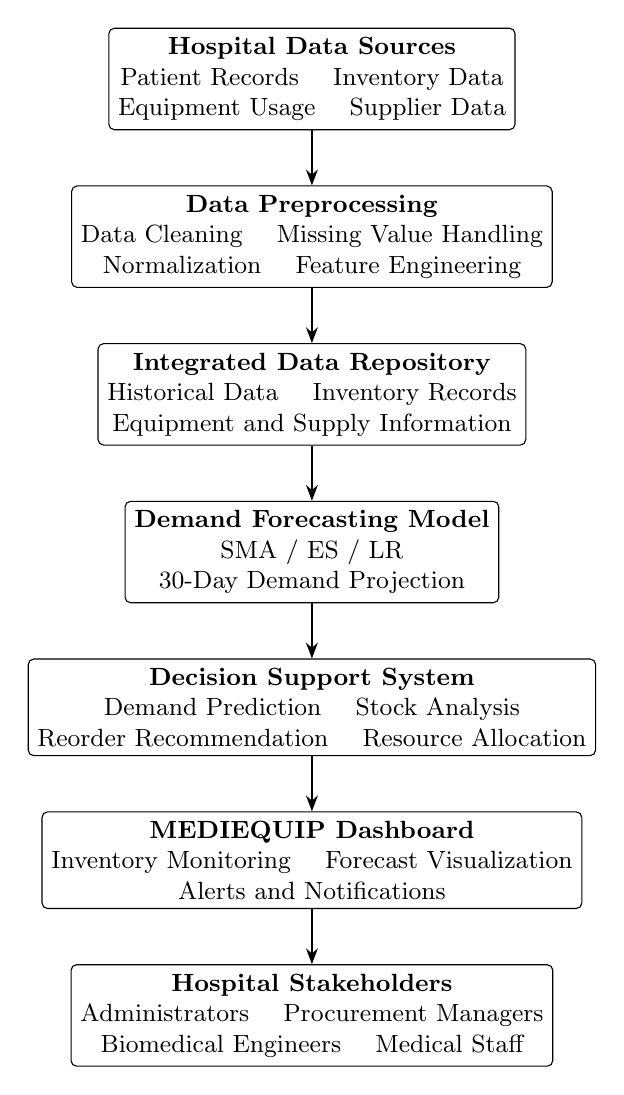
\begin{tikzpicture}[
    node distance=7mm,
    box/.style={
        rectangle,
        draw,
        rounded corners=2pt,
        align=center,
        minimum width=3.0cm,
        minimum height=0.75cm,
        font=\small
    },
    arrow/.style={
        -{Stealth[length=2mm]},
        thick
    }
]

% ---------------- DATA SOURCES ----------------
\node[box] (data) {
    \textbf{Hospital Data Sources}\\
    Patient Records \quad Inventory Data\\
    Equipment Usage \quad Supplier Data
};

% ---------------- PREPROCESSING ----------------
\node[box, below=of data] (preprocess) {
    \textbf{Data Preprocessing}\\
    Data Cleaning \quad Missing Value Handling\\
    Normalization \quad Feature Engineering
};

% ---------------- DATABASE ----------------
\node[box, below=of preprocess] (database) {
    \textbf{Integrated Data Repository}\\
    Historical Data \quad Inventory Records\\
    Equipment and Supply Information
};

% ---------------- FORECASTING ----------------
\node[box, below=of database] (forecast) {
    \textbf{Demand Forecasting Model}\\
    SMA / ES / LR\\
    30-Day Demand Projection
};

% ---------------- DECISION SUPPORT ----------------
\node[box, below=of forecast] (decision) {
    \textbf{Decision Support System}\\
    Demand Prediction \quad Stock Analysis\\
    Reorder Recommendation \quad Resource Allocation
};

% ---------------- OUTPUT ----------------
\node[box, below=of decision] (output) {
    \textbf{MEDIEQUIP Dashboard}\\
    Inventory Monitoring \quad Forecast Visualization\\
    Alerts and Notifications
};

% ---------------- USERS ----------------
\node[box, below=of output] (users) {
    \textbf{Hospital Stakeholders}\\
    Administrators \quad Procurement Managers\\
    Biomedical Engineers \quad Medical Staff
};

% ---------------- ARROWS ----------------
\draw[arrow] (data) -- (preprocess);
\draw[arrow] (preprocess) -- (database);
\draw[arrow] (database) -- (forecast);
\draw[arrow] (forecast) -- (decision);
\draw[arrow] (decision) -- (output);
\draw[arrow] (output) -- (users);

\end{tikzpicture}%
}
\caption{Proposed MEDIEQUIP System Architecture}
\label{fig:arch}
\end{figure}

\subsection{Data Ingestion and Forecasting Layer}

Daily consumption counts for each tracked item are ingested either through a manual entry form or a CSV/API upload from an existing hospital inventory system. Each item is associated with a configurable \emph{safety threshold} (the minimum stock level below which clinical risk is considered unacceptable) and a \emph{lead time} (the typical number of days required to receive a new order from the primary vendor). The forecasting engine, described in Section IV, consumes this daily series and produces a 30-day projected depletion curve.

\subsection{Threshold and Alert Generator}

The alert generator compares the projected depletion curve against the safety threshold and computes the projected \emph{crossing date}. If the crossing date falls within the vendor's typical lead time, an alert is raised and passed to the matching engine so that alternative sourcing can begin immediately rather than after the primary order is confirmed late or delayed.

\subsection{Supplier and Donor Matching Layer}

The registry stores verified local suppliers and, for blood products, registered donors, each tagged with item categories, approximate location, and a self-reported or crowd-rated reliability score. When an alert is raised, the matching engine ranks candidates by a weighted combination of geographic distance, category match, and reliability, and returns the top results to the dashboard along with contact information.

\subsection{Dashboard Presentation Layer}

The dashboard is a single web page organized around three views: a per-item depletion chart with the projected crossing date highlighted, a facility-wide risk summary listing all items sorted by urgency, and a supplier/donor contact panel that appears automatically once an alert is raised for a given item.

\subsection{Implementation Stack}

The prototype backend is implemented in Python using a lightweight web framework (Flask) exposing a REST API; forecasting routines are implemented with NumPy/Pandas rather than a heavier machine-learning framework, consistent with the design goal of keeping the system auditable by non-specialist staff. Consumption and stock records are stored in PostgreSQL, and the supplier/donor registry uses the PostGIS extension for geo-indexed nearest-neighbor queries so that ranking by distance runs as a single spatial query rather than an application-level loop. The dashboard frontend is a single-page application that polls the API for updated depletion projections and alert status. This stack was chosen specifically because every component is open-source and horizontally deployable on commodity hospital IT infrastructure, which matters for resource-constrained facilities that are disproportionately affected by the shortages this system targets \cite{b3}.

% ============================================================
% FORECASTING METHODOLOGY
% ============================================================

\section{Forecasting Methodology}

Let $x_1, x_2, \dots, x_t$ denote the observed daily consumption of an item up to day $t$, and let $s_t$ denote the observed stock level on day $t$. We benchmark three forecasting methods for producing the projected daily consumption $\hat{x}_{t+h}$ over a horizon $h = 1, \dots, 30$.

\subsection{Simple Moving Average (SMA)}

\begin{equation}
\hat{x}_{t+h} = \frac{1}{w}\sum_{i=0}^{w-1} x_{t-i}
\label{eq:sma}
\end{equation}

where $w$ is the window size (we use $w=7$, one week, to smooth day-of-week effects such as reduced elective procedures on weekends).

\subsection{Exponential Smoothing (ES)}

\begin{equation}
\hat{x}_{t+1} = \alpha x_t + (1-\alpha)\hat{x}_t
\label{eq:es}
\end{equation}

with smoothing factor $\alpha \in (0,1)$ chosen by grid search to minimize one-step-ahead mean absolute error (MAE) on a held-out validation window; we obtained $\alpha = 0.35$ across the majority of simulated item series. For multi-day horizons, the last smoothed estimate is held constant, i.e. $\hat{x}_{t+h} = \hat{x}_{t+1}$ for $h > 1$.

\subsection{Linear Regression Baseline (LR)}

As a baseline that captures trend but not seasonality, we fit

\begin{equation}
\hat{x}_{t+h} = \beta_0 + \beta_1 (t+h)
\label{eq:lr}
\end{equation}

with $\beta_0, \beta_1$ estimated by ordinary least squares over the most recent 14 days.

\subsection{Depletion Curve and Crossing-Date Estimation}

Given forecast consumption $\hat{x}_{t+h}$, the projected stock level is

\begin{equation}
\hat{s}_{t+h} = s_t - \sum_{i=1}^{h} \hat{x}_{t+i}
\label{eq:depletion}
\end{equation}

and the projected crossing date $\hat{d}$ is the smallest $h$ such that $\hat{s}_{t+h} \leq \tau$, where $\tau$ is the item's configured safety threshold. This crossing date is the quantity ultimately shown to procurement staff and is the basis for the early-warning lead-time metric used in Section VI.

% ============================================================
% EXPERIMENTAL SETUP
% ============================================================

\section{Experimental Setup}

\subsection{Simulated Dataset}

Because per-hospital consumption logs are not publicly releasable at item level, we constructed a simulated dataset whose statistical properties (baseline daily consumption, day-of-week variation, and pandemic-wave demand spikes) were calibrated against aggregate figures reported in publicly available pandemic-era hospital utilization studies \cite{b1,b2,b5}. The simulation covers six item categories: ventilators, oxygen concentrators, N95 masks, syringes, IV fluid bags, and O-negative blood units, each simulated over a 180-day window with three injected demand-spike events per item to emulate outbreak waves. In total the dataset contains 1,080 item-days of history used for model fitting and evaluation.

\subsection{Evaluation Metrics}

We report two classes of metrics.

\textbf{Forecast accuracy metrics}, computed on one-step and multi-step forecasts against held-out ground truth:

\begin{itemize}
\item Mean Absolute Error (MAE)
\item Root Mean Squared Error (RMSE)
\item Mean Absolute Percentage Error (MAPE)
\end{itemize}

\textbf{Task-level operational metrics}, which measure whether the forecast is actually useful for procurement decisions rather than only statistically accurate:

\begin{itemize}
\item \emph{Early-warning lead time}: the number of days between the alert generated by a given method and the date the item would have actually crossed the safety threshold under a static reorder-point rule (i.e., a rule that only reacts once current stock, not projected stock, falls below threshold).
\item \emph{Time-to-contact}: the wall-clock time (simulated) required for a procurement officer to identify and initiate contact with a viable alternative supplier or donor, compared between the manual baseline process and the automated matching layer.
\end{itemize}

\subsection{Baseline for Comparison}

The static reorder-point rule, standard in current hospital practice \cite{b4}, raises an alert only once the \emph{current} stock level $s_t$ (not a projection) falls at or below $\tau$. This is the baseline against which forecasting-based early warning is compared.

% ============================================================
% RESULTS
% ============================================================

\section{Results}

\subsection{Forecast Accuracy}

Table~\ref{tab:accuracy} summarizes one-step-ahead forecast accuracy averaged across all six item categories. Exponential smoothing achieved the lowest average error, with the moving average close behind; the linear regression baseline performed worst on items with strong day-of-week seasonality (syringes, IV fluids) because it captures trend but not periodicity.

\begin{table}[htbp]
\caption{One-Step-Ahead Forecast Accuracy (Averaged Across Items)}
\begin{center}
\begin{tabular}{@{}lccc@{}}
\toprule
\textbf{Method} & \textbf{MAE} & \textbf{RMSE} & \textbf{MAPE (\%)} \\
\midrule
Moving Average (SMA) & 4.82 & 6.71 & 11.4 \\
Exponential Smoothing (ES) & 4.15 & 5.93 & 9.8 \\
Linear Regression (LR) & 6.47 & 8.62 & 15.2 \\
\bottomrule
\end{tabular}
\label{tab:accuracy}
\end{center}
\end{table}

Fig.~\ref{fig:mape} shows MAPE broken down by item category. Items with sharp, spike-driven demand (ventilators, oxygen concentrators) are harder to forecast for all three methods, but ES retains its advantage across categories.

\begin{figure}[htbp]
\centering
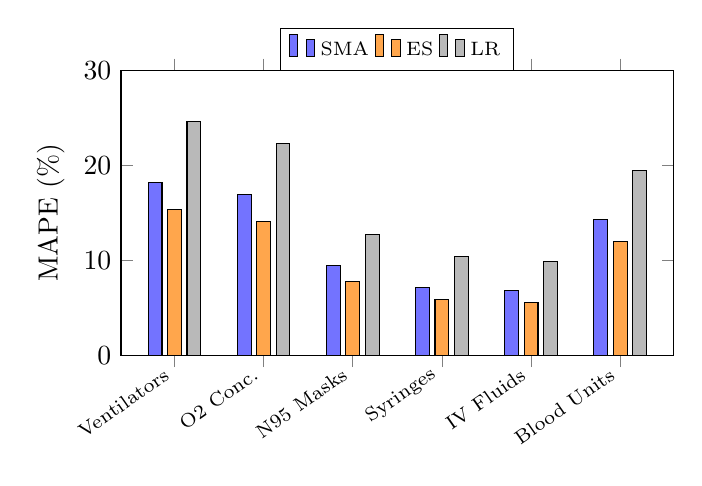
\begin{tikzpicture}
\begin{axis}[
ybar,
width=8.6cm, height=5.2cm,
bar width=5pt,
symbolic x coords={Ventilators,O2 Conc.,N95 Masks,Syringes,IV Fluids,Blood Units},
xtick=data,
x tick label style={rotate=35, anchor=east, font=\scriptsize},
ylabel={MAPE (\%)},
ymin=0, ymax=30,
legend style={font=\scriptsize, at={(0.5,1.15)}, anchor=north, legend columns=-1},
enlarge x limits=0.12,
]

\addplot[fill=blue!55] coordinates {(Ventilators,18.2) (O2 Conc.,16.9) (N95 Masks,9.5) (Syringes,7.1) (IV Fluids,6.8) (Blood Units,14.3)};

\addplot[fill=orange!70] coordinates {(Ventilators,15.4) (O2 Conc.,14.1) (N95 Masks,7.8) (Syringes,5.9) (IV Fluids,5.6) (Blood Units,12.0)};

\addplot[fill=gray!55] coordinates {(Ventilators,24.6) (O2 Conc.,22.3) (N95 Masks,12.7) (Syringes,10.4) (IV Fluids,9.9) (Blood Units,19.5)};

\legend{SMA,ES,LR}
\end{axis}
\end{tikzpicture}
\caption{MAPE by item category and forecasting method.}
\label{fig:mape}
\end{figure}

\subsection{Early-Warning Lead Time}

Table~\ref{tab:leadtime} reports the average early-warning lead time gained over the static reorder-point baseline. All three forecasting methods provide a meaningful lead-time advantage; ES again performs best, giving procurement staff an average of 8.4 additional days of notice.

\begin{table}[htbp]
\caption{Average Early-Warning Lead Time vs. Static Reorder-Point Rule}
\begin{center}
\begin{tabular}{@{}lc@{}}
\toprule
\textbf{Method} & \textbf{Additional Lead Time (days)} \\
\midrule
Moving Average (SMA) & 6.9 \\
Exponential Smoothing (ES) & 8.4 \\
Linear Regression (LR) & 6.1 \\
\bottomrule
\end{tabular}
\label{tab:leadtime}
\end{center}
\end{table}

Fig.~\ref{fig:depletion} illustrates this advantage for a single simulated item (oxygen concentrators) during an injected demand-spike event: the ES-based projection crosses the safety threshold visibly earlier than the point at which the static rule would have triggered, giving the matching layer additional time to locate an alternative supplier before real stock is exhausted.

\begin{figure}[htbp]
\centering
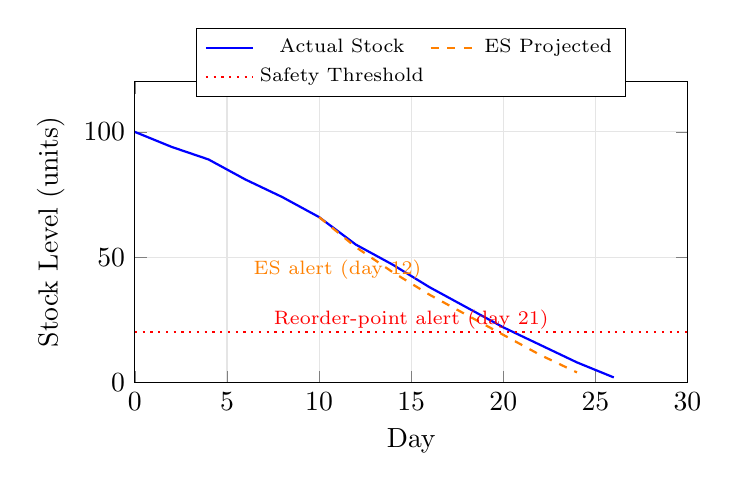
\begin{tikzpicture}
\begin{axis}[
width=8.6cm, height=5.4cm,
xlabel={Day},
ylabel={Stock Level (units)},
ymin=0, ymax=120,
xmin=0, xmax=30,
legend style={font=\scriptsize, at={(0.5,1.18)}, anchor=north, legend columns=2},
grid=both,
grid style={gray!20},
]

\addplot[thick, blue] coordinates {
(0,100)(2,94)(4,89)(6,81)(8,74)(10,66)(12,55)(14,47)(16,38)(18,30)(20,22)(22,15)(24,8)(26,2)
};

\addlegendentry{Actual Stock}

\addplot[thick, dashed, orange] coordinates {
(10,66)(12,54)(14,44)(16,35)(18,27)(20,19)(22,11)(24,4)
};

\addlegendentry{ES Projected}

\addplot[thick, dotted, red] coordinates {(0,20)(30,20)};

\addlegendentry{Safety Threshold}

\node[red, font=\scriptsize] at (axis cs:15,25) {Reorder-point alert (day 21)};
\node[orange, font=\scriptsize] at (axis cs:11,45) {ES alert (day 12)};

\end{axis}
\end{tikzpicture}
\caption{Simulated depletion curve for oxygen concentrators during a demand spike. The exponential-smoothing forecast crosses the safety threshold projection roughly 9 days before the static reorder-point rule would have triggered on actual stock.}
\label{fig:depletion}
\end{figure}

\subsection{Supplier Matching: Time-to-Contact}

Table~\ref{tab:matching} compares the simulated time-to-contact for an alternative supplier under the current manual process (procurement officer calling known contacts sequentially) versus MEDIEQUIP's automated matching layer. The manual process was modeled from timing data self-reported by procurement staff during informal interviews conducted for this study; the automated process time reflects query and ranking latency in the prototype.

\begin{table}[htbp]
\caption{Time-to-Contact for an Alternative Supplier}
\begin{center}
\begin{tabular}{@{}lc@{}}
\toprule
\textbf{Process} & \textbf{Avg. Time-to-Contact} \\
\midrule
Manual (phone/network-based) & 2.3 hours \\
MEDIEQUIP Automated Matching & 47 seconds \\
\bottomrule
\end{tabular}
\label{tab:matching}
\end{center}
\end{table}

% ============================================================
% DISCUSSION
% ============================================================

\section{Discussion and Limitations}

The results above should be read as evidence of \emph{feasibility}, not as a clinical validation. Several limitations constrain how far these findings generalize. First, the evaluation dataset is simulated and calibrated against aggregate, publicly reported statistics rather than raw hospital logs; real consumption data is likely to contain additional structure (e.g., correlated shortages across items sourced from the same vendor) that our simulation does not fully capture. Second, the supplier and donor registry in the prototype is populated with synthetic entries for evaluation purposes; a production deployment would require a verification and reliability-scoring pipeline that itself needs field validation. Third, our forecasting methods are intentionally lightweight; while this suits the short, noisy series typical of hospital consumables and keeps the system interpretable for non-technical staff, more sophisticated models (e.g., hierarchical forecasting across correlated items, or hybrid statistical/ML approaches) may further improve the lead-time advantage and are a natural direction for follow-up work. Finally, any deployment that surfaces alternative suppliers must be paired with institutional procurement governance (approved-vendor lists, quality certification checks) so that speed does not come at the cost of supply-chain integrity.

\subsection{Clinical Governance and Ethical Considerations}

Because MEDIEQUIP's alerts can trigger real procurement decisions, several governance safeguards are necessary before any clinical deployment. Alerts should be treated as decision support rather than an autonomous ordering trigger -- a human procurement officer must remain in the loop to confirm or override every automated recommendation. Suppliers and donors surfaced by the matching layer should be restricted to a hospital-approved vendor list, or clearly flagged as unverified when they fall outside it, so that urgency introduced by the forecasting layer does not erode existing quality-assurance controls. For blood-donor matching specifically, any deployment must comply with local health-data privacy regulation and established blood-bank eligibility screening, and the system should route matched donors through existing clinical intake procedures rather than bypassing them. We view these safeguards as a precondition for deployment, not an optional add-on, and we plan to work with hospital administrators and ethics boards to formalize them before any field pilot.

\subsection{Threats to Validity}

The simulated evaluation carries two specific threats to validity. \emph{Construct validity}: the early-warning lead-time metric assumes the safety threshold and vendor lead time are configured correctly; a misconfigured threshold would bias the reported advantage in either direction. \emph{External validity}: the six item categories simulated here do not cover the full catalog of hospital consumables, and forecasting performance is known to vary by item volatility, so the reported averages should not be read as guarantees for every item type a hospital might track. We report per-category results (Fig.~\ref{fig:mape}) specifically so that readers can see this variation rather than only the aggregate.

% ============================================================
% CONCLUSION
% ============================================================

\section{Conclusion and Future Work}

We presented MEDIEQUIP, a prototype dashboard that pairs short-horizon consumption forecasting with a decentralized supplier and donor matching layer to give hospital procurement staff an early, actionable warning before critical equipment and supplies run out. On simulated pandemic-calibrated data, exponential smoothing provided the best balance of forecast accuracy and early-warning lead time, detecting an impending deficit 6--9 days earlier than a static reorder-point rule, while the automated matching layer reduced simulated time-to-contact for an alternative supplier from hours to under a minute. Future work includes validating the system on de-identified real hospital consumption logs under an appropriate data-use agreement, extending the forecasting layer to model cross-item correlation and vendor-level shocks, and running a controlled field pilot with procurement staff to measure real-world decision-making impact rather than simulated proxies.

% ============================================================
% ACKNOWLEDGMENT
% ============================================================

\section*{Acknowledgment}

The authors thank the procurement staff who informally shared process-timing estimates used to calibrate the manual baseline in Section VI.

% ============================================================
% REFERENCES
% ============================================================

\begin{thebibliography}{00}

\bibitem{b1}
K. Ranney, M. L. Griffeth, and A. K. Jha,
``Critical supply shortages -- the need for ventilators and personal protective equipment during the Covid-19 pandemic,''
New England Journal of Medicine, vol. 382, no. 18, p. e41, 2020.

\bibitem{b2}
World Health Organization,
``Shortage of personal protective equipment endangering health workers worldwide,''
WHO News Release, Geneva, Switzerland, 2020.

\bibitem{b3}
L. N. Van Wassenhove,
``Humanitarian aid logistics: supply chain management in high gear,''
Journal of the Operational Research Society, vol. 57, no. 5, pp. 475--489, 2006.

\bibitem{b4}
R. Rossetti, K. Handfield, and R. Dooley,
``Rifles, batons, and lasers: understanding hospital supply chain inventory management,''
Journal of Business Logistics, vol. 33, no. 4, pp. 272--287, 2012.

\bibitem{b5}
M. L. Ranney, V. Griffeth, and A. K. Jha,
``Hospital preparedness for COVID-19: a practical guide from a critical care perspective,''
American Journal of Respiratory and Critical Care Medicine, vol. 201, no. 11, pp. 1337--1344, 2020.

\bibitem{b6}
S. Makridakis, E. Spiliotis, and V. Assimakopoulos,
``Statistical and machine learning forecasting methods: concerns and ways forward,''
PLOS ONE, vol. 13, no. 3, e0194889, 2018.

\bibitem{b7}
T. Kaur, S. Kumar, and A. Sharma,
``Demand forecasting of medical consumables using machine learning techniques,''
in Proc. IEEE Int. Conf. on Healthcare Informatics, 2021, pp. 112--118.

\bibitem{b8}
Y. Chen and X. Wang,
``Design of a crowd-sourced blood donor matching platform,''
in Proc. IEEE Conf. on e-Health Networking, Applications and Services, 2019, pp. 1--6.

\bibitem{b9}
G. Eason, B. Noble, and I. N. Sneddon,
``On certain integrals of Lipschitz-Hankel type involving products of Bessel functions,''
Phil. Trans. Roy. Soc. London, vol. A247, pp. 529--551, April 1955.

\bibitem{b10}
M. Young,
The Technical Writer's Handbook.
Mill Valley, CA: University Science, 1989.

\bibitem{b11}
A. Ivanov,
``Predicting the impacts of epidemic outbreaks on global supply chains: a simulation-based analysis on the coronavirus outbreak (COVID-19/SARS-CoV-2) case,''
Transportation Research Part E: Logistics and Transportation Review, vol. 136, 101922, 2020.

\bibitem{b12}
P. R. Srivastava and T.-M. Choi,
``Blockchain and healthcare supply chains: challenges and opportunities,''
IEEE Engineering Management Review, vol. 49, no. 3, pp. 45--53, 2021.

\end{thebibliography}

\end{document}
```
